\documentclass{article}
% Chinese
% \documentclass[UTF8, nofonts, mathptmx, 12pt, onecolumn]{article}
% \usepackage{xeCJK}
% \setCJKmainfont{SimSun}
\usepackage{amsmath}
\usepackage{amsfonts}
\usepackage{amssymb}
\usepackage{wasysym}
% \usepackage{ctex}
\usepackage{graphicx}
\usepackage{float}
\usepackage{geometry}
\geometry{a4paper,scale=0.8}
\usepackage{caption}
\usepackage{subcaption}
% \newcommand{\oiint}{\mathop{{\int\!\!\!\!\!\int}\mkern-21mu \bigcirc} {}}
\newcommand*{\dif}{\mathop{}\!\mathrm{d}}
\newcommand*{\md}{\mathop{}\!\mathrm{d}}
\newcommand*{\me}{\mathrm{e}}

\usepackage{parskip}
\setlength{\parindent}{0cm}

\usepackage{bm}
\let\Oldmathbf\mathbf
\renewcommand{\mathbf}[1]{\boldsymbol{\Oldmathbf{#1}}}
\let\eqnarray\align

\author{Xiping Hu}
\usepackage{authblk}
\author{Xiping Hu}
\affil{http://thehxp.tech/}
\title{Homework for Analogue Electronics}

\begin{document}
\maketitle

\begin{figure}[H]
  \centering
  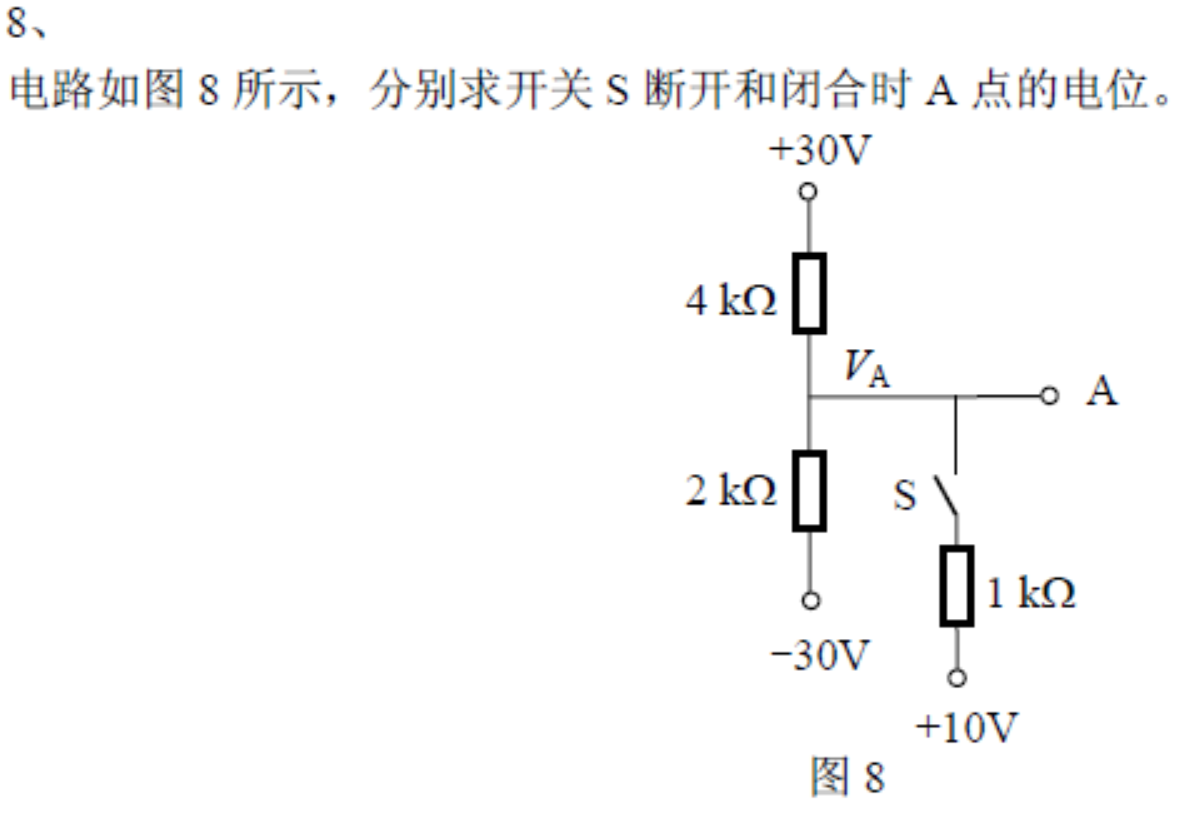
\includegraphics[width=\linewidth]{figures/8}
  \label{fig:}
\end{figure}

\paragraph{Solution}

When $S$ is open

\begin{equation*}
  \begin{aligned}
    V_A = 30 - 4000 \times \dfrac{60}{6000} = - 10 \  \mathrm{V}
  \end{aligned}
\end{equation*}

When $S$ is closed

\begin{figure}[H]
  \centering
  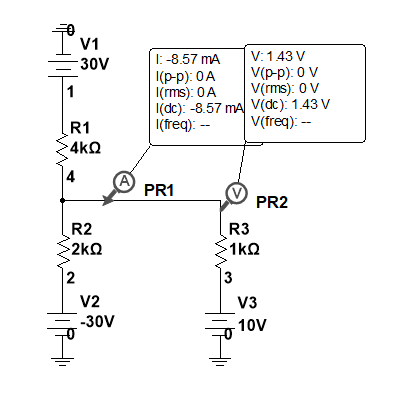
\includegraphics[width=0.5\linewidth]{figures/11}
  \label{fig:}
\end{figure}

\begin{equation*}
  \begin{aligned}
    I_{R1} R_1 + \left( I_{R1} - I_{R3}  \right) R_2 = 60 \  \mathrm{V} \\
    I_{R1} R_1 + I_{R3} R_3 = 20 \  \mathrm{V}
  \end{aligned}
\end{equation*}

\begin{equation*}
  \begin{aligned}
    I_{R3} &= - 8.57 \  \mathrm{\mu A}
  \end{aligned}
\end{equation*}
\begin{equation*}
  \begin{aligned}
    V_A &= 10 \  \mathrm{V} + \left( -8.57 \mathrm{\mu A} \times 1 \mathrm{k \Omega}\right) = 1.43 \ \mathrm{V}
  \end{aligned}
\end{equation*}







\end{document}